\documentclass[12pt]{article}

\usepackage{float}
\usepackage{graphicx}			% Use this package to include images
\usepackage{amsmath}			% A library of many standard math expressions
\usepackage[margin=1in]{geometry}% Sets 1in margins. 
\usepackage{fancyhdr}			% Creates headers and footers
\usepackage{enumerate}          %These two package give custom labels to a list
\usepackage[shortlabels]{enumitem}
\usepackage{matlab-prettifier}
\usepackage{tikz}
\usepackage[utf8]{inputenc}
\usepackage{pgfplots} 
\usepackage{pgfgantt}
\usepackage{pdflscape}
\usepackage{array,multirow}
\usepackage{tabularx,booktabs}
\newcolumntype{Y}{>{\centering\arraybackslash}X}
\usetikzlibrary{shapes.geometric}
\usetikzlibrary{arrows.meta,arrows}
\pgfplotsset{compat=newest} 
\pgfplotsset{plot coordinates/math parser=false}
\newlength\fwidth
\newlength\fheight
\usepackage{float,graphicx}
\pagestyle{fancy}
\fancyhead[l]{}
\fancyhead[c]{Experiment 5}
\fancyhead[r]{}
\fancyfoot[c]{\thepage}
\setlength{\headheight}{20pt}
\begin{document}
\author{}
\date{}
\title{Thermal conductivity by Lee's methord}
\maketitle
\section*{Aim}
To measure the thermal conductivity of bad conductors of heat.
\section*{Analysis}
Newton's law of cooling is given by 
\[\frac{dT}{dt} = -b(T-T_a)\]
For solving this differential equation we shall put $x = T-T_a$
\begin{align*}
    \frac{dx}{dt} &= -bx \\
    \int \frac{dx}{x} &= \int -b dt \\
    \ln |x| &= -bt + c \\
    x &= e^ce^{-bt} \\
    T &= ae^{-bt} +T_a
\end{align*}
We see that the constant $a$ is independent from everything else as it is derived from the constant of integration, which does not depend on the data. 
Performing fitting for the model
\[y = ae^{-bt}+c\]
We obtain the coefficients as listed in the table below.
\begin{table}[H]
    \centering
    \begin{tabular}{|c|c|c|c|c|}
    \hline
        \textbf{Material} & $a$ & $b$ & $c$ & $R^2$ \\ \hline
        Glass & 21.42 & 0.637 & 67.93 & 0.9966 \\ \hline
        Ebonite & 23.48 & 0.257 & 62.40 & 0.9962 \\ \hline
        Wood & 24.48 & 0.115 & 54.13 & 0.9971 \\ \hline
    \end{tabular}
\end{table}

\begin{figure}[H]
    \centering
    \setlength\fwidth{0.75\textwidth}
    \setlength\fheight{0.5\textwidth}
    \caption{Glass}
    % This file was created by matlab2tikz.
%
\definecolor{mycolor1}{rgb}{0.00000,0.44700,0.74100}%
\definecolor{mycolor2}{rgb}{0.85000,0.32500,0.09800}%
\definecolor{mycolor3}{rgb}{0.12941,0.12941,0.12941}%
%
\begin{tikzpicture}

\begin{axis}[%
width=0.951\fwidth,
height=\fheight,
at={(0\fwidth,0\fheight)},
scale only axis,
xmin=0,
xmax=10,
xlabel style={font=\color{mycolor3}},
xlabel={Time (in minutes)},
ymin=60,
ymax=80,
ylabel style={font=\color{mycolor3}},
ylabel={Temperature (in Celcius)},
axis background/.style={fill=white},
xmajorgrids,
ymajorgrids,
legend style={legend cell align=left, align=left}
]
\addplot[only marks, mark=o, mark options={}, mark size=1.5000pt, draw=mycolor1] table[row sep=crcr]{%
x	y\\
0.5	78\\
0.75	76.7\\
1	75.8\\
1.25	75.1\\
1.5	74.6\\
1.75	74.1\\
2	73.6\\
2.25	72.6\\
2.5	72.2\\
2.75	71.6\\
3	71.2\\
3.25	70.9\\
3.5	70.6\\
3.75	70.1\\
4	69.7\\
4.25	69.3\\
4.5	68.8\\
4.75	68.5\\
5	68.1\\
5.25	67.7\\
5.5	67.1\\
5.75	66.8\\
6	66.3\\
6.25	66\\
6.5	65.7\\
6.75	65.7\\
7	65.4\\
7.25	65\\
7.5	64.6\\
7.75	64.2\\
8	63.9\\
8.25	63.5\\
8.5	63.1\\
8.75	62.9\\
9	62.5\\
};
\addlegendentry{Data}

\addplot [color=mycolor2]
  table[row sep=crcr]{%
-1	81.5933908962963\\
-0.9	81.2793475453082\\
-0.8	80.9688953786577\\
-0.7	80.6619933300243\\
-0.6	80.3586008026937\\
-0.5	80.0586776641875\\
-0.4	79.7621842409552\\
-0.3	79.4690813131255\\
-0.2	79.1793301093187\\
-0.1	78.8928923015181\\
0	78.60973\\
0.1	78.3298057483213\\
0.2	78.0530825183652\\
0.3	77.7795237054433\\
0.4	77.5090931234528\\
0.5	77.2417550000909\\
0.6	76.9774739721219\\
0.7	76.7162150807\\
0.8	76.4579437667448\\
0.9	76.2026258663697\\
1	75.950227606363\\
1.1	75.7007155997202\\
1.2	75.4540568412277\\
1.3	75.2102187030969\\
1.4	74.9691689306482\\
1.5	74.7308756380445\\
1.6	74.495307304073\\
1.7	74.2624327679761\\
1.8	74.0322212253292\\
1.9	73.8046422239658\\
2	73.5796656599498\\
2.1	73.3572617735928\\
2.2	73.1374011455178\\
2.3	72.9200546927678\\
2.4	72.7051936649585\\
2.5	72.492789640475\\
2.6	72.2828145227128\\
2.7	72.0752405363608\\
2.8	71.8700402237273\\
2.9	71.6671864411079\\
3	71.466652355195\\
3.1	71.2684114395283\\
3.2	71.0724374709859\\
3.3	70.8787045263156\\
3.4	70.6871869787057\\
3.5	70.497859494395\\
3.6	70.310697029322\\
3.7	70.1256748258118\\
3.8	69.9427684093014\\
3.9	69.7619535851019\\
4	69.5832064351985\\
4.1	69.4065033150863\\
4.2	69.2318208506427\\
4.3	69.0591359350357\\
4.4	68.8884257256669\\
4.5	68.7196676411505\\
4.6	68.5528393583257\\
4.7	68.3879188093041\\
4.8	68.2248841785507\\
4.9	68.0637138999978\\
5	67.9043866541925\\
5.1	67.7468813654765\\
5.2	67.5911771991985\\
5.3	67.4372535589578\\
5.4	67.2850900838799\\
5.5	67.1346666459234\\
5.6	66.9859633472176\\
5.7	66.8389605174298\\
5.8	66.6936387111639\\
5.9	66.5499787053882\\
6	66.4079614968922\\
6.1	66.267568299773\\
6.2	66.1287805429507\\
6.3	65.9915798677111\\
6.4	65.8559481252781\\
6.5	65.7218673744124\\
6.6	65.5893198790382\\
6.7	65.4582881058976\\
6.8	65.3287547222307\\
6.9	65.2007025934836\\
7	65.0741147810409\\
7.1	64.948974539986\\
7.2	64.8252653168853\\
7.3	64.7029707475993\\
7.4	64.5820746551172\\
7.5	64.4625610474178\\
7.6	64.3444141153533\\
7.7	64.2276182305587\\
7.8	64.1121579433841\\
7.9	63.9980179808515\\
8	63.8851832446338\\
8.1	63.7736388090584\\
8.2	63.663369919132\\
8.3	63.5543619885898\\
8.4	63.4466005979651\\
8.5	63.3400714926826\\
8.6	63.2347605811724\\
8.7	63.1306539330061\\
8.8	63.0277377770542\\
8.9	62.9259984996645\\
9	62.8254226428609\\
9.1	62.7259969025638\\
9.2	62.6277081268297\\
9.3	62.5305433141117\\
9.4	62.4344896115399\\
9.5	62.3395343132208\\
9.6	62.2456648585568\\
9.7	62.1528688305848\\
9.8	62.0611339543334\\
9.9	61.9704480951995\\
10	61.8807992573429\\
};
\addlegendentry{Fit}

\addplot [color=black, dashed]
  table[row sep=crcr]{%
-1	78.52891\\
-0.9	78.361649\\
-0.8	78.194388\\
-0.7	78.027127\\
-0.6	77.859866\\
-0.5	77.692605\\
-0.4	77.525344\\
-0.3	77.358083\\
-0.2	77.190822\\
-0.1	77.023561\\
0	76.8563\\
0.1	76.689039\\
0.2	76.521778\\
0.3	76.354517\\
0.4	76.187256\\
0.5	76.019995\\
0.6	75.852734\\
0.7	75.685473\\
0.8	75.518212\\
0.9	75.350951\\
1	75.18369\\
1.1	75.016429\\
1.2	74.849168\\
1.3	74.681907\\
1.4	74.514646\\
1.5	74.347385\\
1.6	74.180124\\
1.7	74.012863\\
1.8	73.845602\\
1.9	73.678341\\
2	73.51108\\
2.1	73.343819\\
2.2	73.176558\\
2.3	73.009297\\
2.4	72.842036\\
2.5	72.674775\\
2.6	72.507514\\
2.7	72.340253\\
2.8	72.172992\\
2.9	72.005731\\
3	71.83847\\
3.1	71.671209\\
3.2	71.503948\\
3.3	71.336687\\
3.4	71.169426\\
3.5	71.002165\\
3.6	70.834904\\
3.7	70.667643\\
3.8	70.500382\\
3.9	70.333121\\
4	70.16586\\
4.1	69.998599\\
4.2	69.831338\\
4.3	69.664077\\
4.4	69.496816\\
4.5	69.329555\\
4.6	69.162294\\
4.7	68.995033\\
4.8	68.827772\\
4.9	68.660511\\
5	68.49325\\
5.1	68.325989\\
5.2	68.158728\\
5.3	67.991467\\
5.4	67.824206\\
5.5	67.656945\\
5.6	67.489684\\
5.7	67.322423\\
5.8	67.155162\\
5.9	66.987901\\
6	66.82064\\
6.1	66.653379\\
6.2	66.486118\\
6.3	66.318857\\
6.4	66.151596\\
6.5	65.984335\\
6.6	65.817074\\
6.7	65.649813\\
6.8	65.482552\\
6.9	65.315291\\
7	65.14803\\
7.1	64.980769\\
7.2	64.813508\\
7.3	64.646247\\
7.4	64.478986\\
7.5	64.311725\\
7.6	64.144464\\
7.7	63.977203\\
7.8	63.809942\\
7.9	63.642681\\
8	63.47542\\
8.1	63.308159\\
8.2	63.140898\\
8.3	62.973637\\
8.4	62.806376\\
8.5	62.639115\\
8.6	62.471854\\
8.7	62.304593\\
8.8	62.137332\\
8.9	61.970071\\
9	61.80281\\
9.1	61.635549\\
9.2	61.468288\\
9.3	61.301027\\
9.4	61.133766\\
9.5	60.966505\\
9.6	60.799244\\
9.7	60.631983\\
9.8	60.464722\\
9.9	60.297461\\
10	60.1302\\
};
\addlegendentry{Linear}

\end{axis}
\end{tikzpicture}%
    \caption{Ebonite}
    % This file was created by matlab2tikz.
%
\definecolor{mycolor1}{rgb}{0.00000,0.44700,0.74100}%
\definecolor{mycolor2}{rgb}{0.85000,0.32500,0.09800}%
\definecolor{mycolor3}{rgb}{0.12941,0.12941,0.12941}%
%
\begin{tikzpicture}

\begin{axis}[%
width=0.951\fwidth,
height=\fheight,
at={(0\fwidth,0\fheight)},
scale only axis,
xmin=-0.25,
xmax=4.5,
xlabel style={font=\color{mycolor3}},
xlabel={Time (in minutes)},
ymin=65,
ymax=95,
ylabel style={font=\color{mycolor3}},
ylabel={Temperature (in Celcius)},
axis background/.style={fill=white},
xmajorgrids,
ymajorgrids,
legend style={legend cell align=left, align=left}
]
\addplot[only marks, mark=o, mark options={}, mark size=1.5000pt, draw=mycolor1] table[row sep=crcr]{%
x	y\\
0	89.5\\
0.25	86.5\\
0.5	83.5\\
0.75	80.5\\
1	79\\
1.25	77.5\\
1.5	76\\
1.75	75\\
2	74\\
2.25	73.5\\
2.5	72.5\\
2.75	72\\
3	71.5\\
3.25	71\\
3.5	70\\
3.75	69.5\\
4	69\\
};
\addlegendentry{Data}

\addplot [color=mycolor2]
  table[row sep=crcr]{%
-1	108.444036531024\\
-0.9	105.942232307116\\
-0.8	103.594906416977\\
-0.7	101.392520322229\\
-0.6	99.3261244584442\\
-0.5	97.3873218679037\\
-0.4	95.5682340779188\\
-0.3	93.8614690860536\\
-0.2	92.2600913221575\\
-0.1	90.7575934651453\\
0	89.34787\\
0.1	88.0251924075453\\
0.2	86.7841858861696\\
0.3	85.6198075109081\\
0.4	84.5273257411317\\
0.5	83.5023011935695\\
0.6	82.5405686025348\\
0.7	81.6382198940497\\
0.8	80.7915883050872\\
0.9	79.9972334833991\\
1	79.2519275073814\\
1.1	78.5526417691678\\
1.2	77.8965346676498\\
1.3	77.2809400614135\\
1.4	76.7033564346696\\
1.5	76.1614367321524\\
1.6	75.6529788216818\\
1.7	75.17591654563\\
1.8	74.7283113249323\\
1.9	74.3083442815224\\
2	73.9143088471825\\
2.1	73.5446038287725\\
2.2	73.1977269016593\\
2.3	72.8722685049056\\
2.4	72.5669061134114\\
2.5	72.2803988637317\\
2.6	72.011582511733\\
2.7	71.7593647015986\\
2.8	71.5227205269567\\
2.9	71.3006883660948\\
3	71.0923659743369\\
3.1	70.8969068177027\\
3.2	70.7135166329522\\
3.3	70.5414502000361\\
3.4	70.3800083138374\\
3.5	70.2285349428974\\
3.6	70.0864145635823\\
3.7	69.9530696588553\\
3.8	69.8279583714921\\
3.9	69.7105723022027\\
4	69.6004344437118\\
4.1	69.4970972424034\\
4.2	69.4001407796524\\
4.3	69.3091710654531\\
4.4	69.2238184374104\\
4.5	69.1437360585891\\
4.6	69.0685985081146\\
4.7	68.9981004588008\\
4.8	68.9319554364298\\
4.9	68.8698946556414\\
5	68.8116659277039\\
5.1	68.7570326357255\\
5.2	68.7057727731436\\
5.3	68.657678041584\\
5.4	68.6125530044247\\
5.5	68.5702142926242\\
5.6	68.5304898595871\\
5.7	68.49321828204\\
5.8	68.4582481040754\\
5.9	68.4254372216991\\
6	68.3946523053799\\
6.1	68.3657682582545\\
6.2	68.3386677077872\\
6.3	68.3132405288173\\
6.4	68.2893833960573\\
6.5	68.2669993642227\\
6.6	68.2459974740871\\
6.7	68.226292382863\\
6.8	68.2078040174043\\
6.9	68.190457248823\\
7	68.1741815871978\\
7.1	68.158910895132\\
7.2	68.1445831189999\\
7.3	68.1311400367869\\
7.4	68.1185270214997\\
7.5	68.1066928191854\\
7.6	68.0955893406574\\
7.7	68.085171466081\\
7.8	68.0753968616256\\
7.9	68.0662258074382\\
8	68.0576210362381\\
8.1	68.0495475818792\\
8.2	68.0419726372618\\
8.3	68.0348654210189\\
8.4	68.0281970524335\\
8.5	68.0219404340794\\
8.6	68.0160701417092\\
8.7	68.0105623209407\\
8.8	68.0053945903226\\
8.9	68.0005459503863\\
9	67.9959966983122\\
9.1	67.9917283478665\\
9.2	67.9877235542804\\
9.3	67.9839660437689\\
9.4	67.9804405474003\\
9.5	67.9771327390505\\
9.6	67.974029177187\\
9.7	67.9711172502488\\
9.8	67.9683851253979\\
9.9	67.9658217004358\\
10	67.9634165586892\\
};
\addlegendentry{Fit}

\addplot [color=black, dashed]
  table[row sep=crcr]{%
-1	89.63235\\
-0.9	89.174997\\
-0.8	88.717644\\
-0.7	88.260291\\
-0.6	87.802938\\
-0.5	87.345585\\
-0.4	86.888232\\
-0.3	86.430879\\
-0.2	85.973526\\
-0.1	85.516173\\
0	85.05882\\
0.1	84.601467\\
0.2	84.144114\\
0.3	83.686761\\
0.4	83.229408\\
0.5	82.772055\\
0.6	82.314702\\
0.7	81.857349\\
0.8	81.399996\\
0.9	80.942643\\
1	80.48529\\
1.1	80.027937\\
1.2	79.570584\\
1.3	79.113231\\
1.4	78.655878\\
1.5	78.198525\\
1.6	77.741172\\
1.7	77.283819\\
1.8	76.826466\\
1.9	76.369113\\
2	75.91176\\
2.1	75.454407\\
2.2	74.997054\\
2.3	74.539701\\
2.4	74.082348\\
2.5	73.624995\\
2.6	73.167642\\
2.7	72.710289\\
2.8	72.252936\\
2.9	71.795583\\
3	71.33823\\
3.1	70.880877\\
3.2	70.423524\\
3.3	69.966171\\
3.4	69.508818\\
3.5	69.051465\\
3.6	68.594112\\
3.7	68.136759\\
3.8	67.679406\\
3.9	67.222053\\
4	66.7647\\
4.1	66.307347\\
4.2	65.849994\\
4.3	65.392641\\
4.4	64.935288\\
4.5	64.477935\\
4.6	64.020582\\
4.7	63.563229\\
4.8	63.105876\\
4.9	62.648523\\
5	62.19117\\
5.1	61.733817\\
5.2	61.276464\\
5.3	60.819111\\
5.4	60.361758\\
5.5	59.904405\\
5.6	59.447052\\
5.7	58.989699\\
5.8	58.532346\\
5.9	58.074993\\
6	57.61764\\
6.1	57.160287\\
6.2	56.702934\\
6.3	56.245581\\
6.4	55.788228\\
6.5	55.330875\\
6.6	54.873522\\
6.7	54.416169\\
6.8	53.958816\\
6.9	53.501463\\
7	53.04411\\
7.1	52.586757\\
7.2	52.129404\\
7.3	51.672051\\
7.4	51.214698\\
7.5	50.757345\\
7.6	50.299992\\
7.7	49.842639\\
7.8	49.385286\\
7.9	48.927933\\
8	48.47058\\
8.1	48.013227\\
8.2	47.555874\\
8.3	47.098521\\
8.4	46.641168\\
8.5	46.183815\\
8.6	45.726462\\
8.7	45.269109\\
8.8	44.811756\\
8.9	44.354403\\
9	43.89705\\
9.1	43.439697\\
9.2	42.982344\\
9.3	42.524991\\
9.4	42.067638\\
9.5	41.610285\\
9.6	41.152932\\
9.7	40.695579\\
9.8	40.238226\\
9.9	39.780873\\
10	39.32352\\
};
\addlegendentry{Linear}

\end{axis}
\end{tikzpicture}%
\end{figure}
\begin{figure}[H]
    \centering
    \setlength\fwidth{0.75\textwidth}
    \setlength\fheight{0.5\textwidth}
    \caption{Wood}
    % This file was created by matlab2tikz.
%
\definecolor{mycolor1}{rgb}{0.00000,0.44700,0.74100}%
\definecolor{mycolor2}{rgb}{0.85000,0.32500,0.09800}%
\definecolor{mycolor3}{rgb}{0.49400,0.18400,0.55600}%
\definecolor{mycolor4}{rgb}{0.46600,0.67400,0.18800}%
\definecolor{mycolor5}{rgb}{0.63500,0.07800,0.18400}%
\definecolor{mycolor6}{rgb}{0.92900,0.69400,0.12500}%
\definecolor{mycolor7}{rgb}{0.30100,0.74500,0.93300}%
\definecolor{mycolor8}{rgb}{0.12941,0.12941,0.12941}%
%
\begin{tikzpicture}

\begin{axis}[%
width=0.951\fwidth,
height=\fheight,
at={(0\fwidth,0\fheight)},
scale only axis,
xmin=-0.5,
xmax=7,
xlabel style={font=\color{mycolor8}},
xlabel={Time (in minutes)},
ymin=60,
ymax=90,
ylabel style={font=\color{mycolor8}},
ylabel={Temperature (in Celcius)},
axis background/.style={fill=white},
xmajorgrids,
ymajorgrids,
legend style={legend cell align=left, align=left}
]
\addplot[only marks, mark=o, mark options={}, mark size=1.5000pt, draw=mycolor1] table[row sep=crcr]{%
x	y\\
0	86\\
0.25	85\\
0.5	83.5\\
0.75	81.5\\
1	80\\
1.25	79\\
1.5	78\\
1.75	77\\
2	76\\
2.25	75.5\\
2.5	75\\
2.75	74\\
3	73\\
3.25	73\\
3.5	72.5\\
3.75	71.5\\
4	71\\
4.25	70.5\\
4.5	70.5\\
4.75	69.5\\
5	69\\
5.25	68.5\\
5.5	68\\
5.75	67.5\\
6	67\\
6.25	67\\
6.5	66.5\\
};
\addlegendentry{Data}

\addplot [color=mycolor2]
  table[row sep=crcr]{%
-1	92.760185392473\\
-0.9	91.9897498043572\\
-0.8	91.2388658984899\\
-0.7	90.5070375032449\\
-0.6	89.7937810385611\\
-0.5	89.098625196401\\
-0.4	88.421110629318\\
-0.3	87.7607896469276\\
-0.2	87.1172259200805\\
-0.1	86.4899941925442\\
0	85.87868\\
0.1	85.2828793961725\\
0.2	84.7021986859081\\
0.3	84.1362541650281\\
0.4	83.5846718667834\\
0.5	83.0470873147429\\
0.6	82.5231452819545\\
0.7	82.0124995562159\\
0.8	81.5148127113044\\
0.9	81.0297558840103\\
1	80.5570085568302\\
1.1	80.0962583461742\\
1.2	79.6472007959478\\
1.3	79.2095391763726\\
1.4	78.782984287912\\
1.5	78.3672542701732\\
1.6	77.9620744156582\\
1.7	77.5671769882418\\
1.8	77.1823010462562\\
1.9	76.8071922700647\\
2	76.4416027940119\\
2.1	76.0852910426377\\
2.2	75.7380215710489\\
2.3	75.3995649093405\\
2.4	75.0696974109661\\
2.5	74.7482011049559\\
2.6	74.4348635518852\\
2.7	74.1294777034978\\
2.8	73.831841765892\\
2.9	73.5417590661787\\
3	73.2590379225229\\
3.1	72.9834915174837\\
3.2	72.7149377745687\\
3.3	72.4531992379202\\
3.4	72.1981029550561\\
3.5	71.9494803625853\\
3.6	71.7071671748236\\
3.7	71.4710032752372\\
3.8	71.2408326106395\\
3.9	71.0165030880745\\
4	70.7978664743157\\
4.1	70.5847782979162\\
4.2	70.3770977537448\\
4.3	70.1746876099436\\
4.4	69.9774141172481\\
4.5	69.7851469206073\\
4.6	69.5977589730479\\
4.7	69.4151264517232\\
4.8	69.2371286760934\\
4.9	69.0636480281817\\
5	68.8945698748543\\
5.1	68.7297824920728\\
5.2	68.5691769910689\\
5.3	68.4126472463923\\
5.4	68.2600898257848\\
5.5	68.1114039218341\\
5.6	67.9664912853619\\
5.7	67.8252561605023\\
5.8	67.6876052214283\\
5.9	67.5534475106832\\
6	67.4226943790776\\
6.1	67.2952594271117\\
6.2	67.1710584478837\\
6.3	67.0500093714471\\
6.4	66.9320322105807\\
6.5	66.8170490079341\\
6.6	66.7049837845148\\
6.7	66.5957624894825\\
6.8	66.4893129512177\\
6.9	66.3855648296316\\
7	66.284449569687\\
7.1	66.1859003560977\\
7.2	66.0898520691786\\
7.3	65.9962412418153\\
7.4	65.9050060175262\\
7.5	65.8160861095889\\
7.6	65.7294227612036\\
7.7	65.6449587066677\\
7.8	65.5626381335352\\
7.9	65.4824066457374\\
8	65.4042112276382\\
8.1	65.3280002090029\\
8.2	65.2537232308548\\
8.3	65.1813312121991\\
8.4	65.1107763175911\\
8.5	65.042011925527\\
8.6	64.9749925976375\\
8.7	64.9096740486628\\
8.8	64.8460131171893\\
8.9	64.7839677371299\\
9	64.7234969099269\\
9.1	64.6645606774609\\
9.2	64.6071200956475\\
9.3	64.5511372087032\\
9.4	64.4965750240652\\
9.5	64.4433974879473\\
9.6	64.3915694615157\\
9.7	64.3410566976707\\
9.8	64.2918258184159\\
9.9	64.2438442928032\\
10	64.1970804154366\\
};
\addlegendentry{Fit}

\addplot [color=black, dashed]
  table[row sep=crcr]{%
-1	85.90496\\
-0.9	85.622665\\
-0.8	85.34037\\
-0.7	85.058075\\
-0.6	84.77578\\
-0.5	84.493485\\
-0.4	84.21119\\
-0.3	83.928895\\
-0.2	83.6466\\
-0.1	83.364305\\
0	83.08201\\
0.1	82.799715\\
0.2	82.51742\\
0.3	82.235125\\
0.4	81.95283\\
0.5	81.670535\\
0.6	81.38824\\
0.7	81.105945\\
0.8	80.82365\\
0.9	80.541355\\
1	80.25906\\
1.1	79.976765\\
1.2	79.69447\\
1.3	79.412175\\
1.4	79.12988\\
1.5	78.847585\\
1.6	78.56529\\
1.7	78.282995\\
1.8	78.0007\\
1.9	77.718405\\
2	77.43611\\
2.1	77.153815\\
2.2	76.87152\\
2.3	76.589225\\
2.4	76.30693\\
2.5	76.024635\\
2.6	75.74234\\
2.7	75.460045\\
2.8	75.17775\\
2.9	74.895455\\
3	74.61316\\
3.1	74.330865\\
3.2	74.04857\\
3.3	73.766275\\
3.4	73.48398\\
3.5	73.201685\\
3.6	72.91939\\
3.7	72.637095\\
3.8	72.3548\\
3.9	72.072505\\
4	71.79021\\
4.1	71.507915\\
4.2	71.22562\\
4.3	70.943325\\
4.4	70.66103\\
4.5	70.378735\\
4.6	70.09644\\
4.7	69.814145\\
4.8	69.53185\\
4.9	69.249555\\
5	68.96726\\
5.1	68.684965\\
5.2	68.40267\\
5.3	68.120375\\
5.4	67.83808\\
5.5	67.555785\\
5.6	67.27349\\
5.7	66.991195\\
5.8	66.7089\\
5.9	66.426605\\
6	66.14431\\
6.1	65.862015\\
6.2	65.57972\\
6.3	65.297425\\
6.4	65.01513\\
6.5	64.732835\\
6.6	64.45054\\
6.7	64.168245\\
6.8	63.88595\\
6.9	63.603655\\
7	63.32136\\
7.1	63.039065\\
7.2	62.75677\\
7.3	62.474475\\
7.4	62.19218\\
7.5	61.909885\\
7.6	61.62759\\
7.7	61.345295\\
7.8	61.063\\
7.9	60.780705\\
8	60.49841\\
8.1	60.216115\\
8.2	59.93382\\
8.3	59.651525\\
8.4	59.36923\\
8.5	59.086935\\
8.6	58.80464\\
8.7	58.522345\\
8.8	58.24005\\
8.9	57.957755\\
9	57.67546\\
9.1	57.393165\\
9.2	57.11087\\
9.3	56.828575\\
9.4	56.54628\\
9.5	56.263985\\
9.6	55.98169\\
9.7	55.699395\\
9.8	55.4171\\
9.9	55.134805\\
10	54.85251\\
};
\addlegendentry{Linear}

\addplot[only marks, mark=o, mark options={}, mark size=1.5000pt, draw=mycolor3, forget plot] table[row sep=crcr]{%
x	y\\
0	86\\
0.25	85\\
0.5	83.5\\
0.75	81.5\\
1	80\\
1.25	79\\
1.5	78\\
1.75	77\\
2	76\\
2.25	75.5\\
2.5	75\\
2.75	74\\
3	73\\
3.25	73\\
3.5	72.5\\
3.75	71.5\\
4	71\\
4.25	70.5\\
4.5	70.5\\
4.75	69.5\\
5	69\\
5.25	68.5\\
5.5	68\\
5.75	67.5\\
6	67\\
6.25	67\\
6.5	66.5\\
};
\addplot [color=mycolor4, forget plot]
  table[row sep=crcr]{%
-1	92.760185392473\\
-0.9	91.9897498043572\\
-0.8	91.2388658984899\\
-0.7	90.5070375032449\\
-0.6	89.7937810385611\\
-0.5	89.098625196401\\
-0.4	88.421110629318\\
-0.3	87.7607896469276\\
-0.2	87.1172259200805\\
-0.1	86.4899941925442\\
0	85.87868\\
0.1	85.2828793961725\\
0.2	84.7021986859081\\
0.3	84.1362541650281\\
0.4	83.5846718667834\\
0.5	83.0470873147429\\
0.6	82.5231452819545\\
0.7	82.0124995562159\\
0.8	81.5148127113044\\
0.9	81.0297558840103\\
1	80.5570085568302\\
1.1	80.0962583461742\\
1.2	79.6472007959478\\
1.3	79.2095391763726\\
1.4	78.782984287912\\
1.5	78.3672542701732\\
1.6	77.9620744156582\\
1.7	77.5671769882418\\
1.8	77.1823010462562\\
1.9	76.8071922700647\\
2	76.4416027940119\\
2.1	76.0852910426377\\
2.2	75.7380215710489\\
2.3	75.3995649093405\\
2.4	75.0696974109661\\
2.5	74.7482011049559\\
2.6	74.4348635518852\\
2.7	74.1294777034978\\
2.8	73.831841765892\\
2.9	73.5417590661787\\
3	73.2590379225229\\
3.1	72.9834915174837\\
3.2	72.7149377745687\\
3.3	72.4531992379202\\
3.4	72.1981029550561\\
3.5	71.9494803625853\\
3.6	71.7071671748236\\
3.7	71.4710032752372\\
3.8	71.2408326106395\\
3.9	71.0165030880745\\
4	70.7978664743157\\
4.1	70.5847782979162\\
4.2	70.3770977537448\\
4.3	70.1746876099436\\
4.4	69.9774141172481\\
4.5	69.7851469206073\\
4.6	69.5977589730479\\
4.7	69.4151264517232\\
4.8	69.2371286760934\\
4.9	69.0636480281817\\
5	68.8945698748543\\
5.1	68.7297824920728\\
5.2	68.5691769910689\\
5.3	68.4126472463923\\
5.4	68.2600898257848\\
5.5	68.1114039218341\\
5.6	67.9664912853619\\
5.7	67.8252561605023\\
5.8	67.6876052214283\\
5.9	67.5534475106832\\
6	67.4226943790776\\
6.1	67.2952594271117\\
6.2	67.1710584478837\\
6.3	67.0500093714471\\
6.4	66.9320322105807\\
6.5	66.8170490079341\\
6.6	66.7049837845148\\
6.7	66.5957624894825\\
6.8	66.4893129512177\\
6.9	66.3855648296316\\
7	66.284449569687\\
7.1	66.1859003560977\\
7.2	66.0898520691786\\
7.3	65.9962412418153\\
7.4	65.9050060175262\\
7.5	65.8160861095889\\
7.6	65.7294227612036\\
7.7	65.6449587066677\\
7.8	65.5626381335352\\
7.9	65.4824066457374\\
8	65.4042112276382\\
8.1	65.3280002090029\\
8.2	65.2537232308548\\
8.3	65.1813312121991\\
8.4	65.1107763175911\\
8.5	65.042011925527\\
8.6	64.9749925976375\\
8.7	64.9096740486628\\
8.8	64.8460131171893\\
8.9	64.7839677371299\\
9	64.7234969099269\\
9.1	64.6645606774609\\
9.2	64.6071200956475\\
9.3	64.5511372087032\\
9.4	64.4965750240652\\
9.5	64.4433974879473\\
9.6	64.3915694615157\\
9.7	64.3410566976707\\
9.8	64.2918258184159\\
9.9	64.2438442928032\\
10	64.1970804154366\\
};
\addplot [color=black, dashed, forget plot]
  table[row sep=crcr]{%
-1	85.90496\\
-0.9	85.622665\\
-0.8	85.34037\\
-0.7	85.058075\\
-0.6	84.77578\\
-0.5	84.493485\\
-0.4	84.21119\\
-0.3	83.928895\\
-0.2	83.6466\\
-0.1	83.364305\\
0	83.08201\\
0.1	82.799715\\
0.2	82.51742\\
0.3	82.235125\\
0.4	81.95283\\
0.5	81.670535\\
0.6	81.38824\\
0.7	81.105945\\
0.8	80.82365\\
0.9	80.541355\\
1	80.25906\\
1.1	79.976765\\
1.2	79.69447\\
1.3	79.412175\\
1.4	79.12988\\
1.5	78.847585\\
1.6	78.56529\\
1.7	78.282995\\
1.8	78.0007\\
1.9	77.718405\\
2	77.43611\\
2.1	77.153815\\
2.2	76.87152\\
2.3	76.589225\\
2.4	76.30693\\
2.5	76.024635\\
2.6	75.74234\\
2.7	75.460045\\
2.8	75.17775\\
2.9	74.895455\\
3	74.61316\\
3.1	74.330865\\
3.2	74.04857\\
3.3	73.766275\\
3.4	73.48398\\
3.5	73.201685\\
3.6	72.91939\\
3.7	72.637095\\
3.8	72.3548\\
3.9	72.072505\\
4	71.79021\\
4.1	71.507915\\
4.2	71.22562\\
4.3	70.943325\\
4.4	70.66103\\
4.5	70.378735\\
4.6	70.09644\\
4.7	69.814145\\
4.8	69.53185\\
4.9	69.249555\\
5	68.96726\\
5.1	68.684965\\
5.2	68.40267\\
5.3	68.120375\\
5.4	67.83808\\
5.5	67.555785\\
5.6	67.27349\\
5.7	66.991195\\
5.8	66.7089\\
5.9	66.426605\\
6	66.14431\\
6.1	65.862015\\
6.2	65.57972\\
6.3	65.297425\\
6.4	65.01513\\
6.5	64.732835\\
6.6	64.45054\\
6.7	64.168245\\
6.8	63.88595\\
6.9	63.603655\\
7	63.32136\\
7.1	63.039065\\
7.2	62.75677\\
7.3	62.474475\\
7.4	62.19218\\
7.5	61.909885\\
7.6	61.62759\\
7.7	61.345295\\
7.8	61.063\\
7.9	60.780705\\
8	60.49841\\
8.1	60.216115\\
8.2	59.93382\\
8.3	59.651525\\
8.4	59.36923\\
8.5	59.086935\\
8.6	58.80464\\
8.7	58.522345\\
8.8	58.24005\\
8.9	57.957755\\
9	57.67546\\
9.1	57.393165\\
9.2	57.11087\\
9.3	56.828575\\
9.4	56.54628\\
9.5	56.263985\\
9.6	55.98169\\
9.7	55.699395\\
9.8	55.4171\\
9.9	55.134805\\
10	54.85251\\
};
\addplot[only marks, mark=o, mark options={}, mark size=1.5000pt, draw=mycolor5, forget plot] table[row sep=crcr]{%
x	y\\
0	86\\
0.25	85\\
0.5	83.5\\
0.75	81.5\\
1	80\\
1.25	79\\
1.5	78\\
1.75	77\\
2	76\\
2.25	75.5\\
2.5	75\\
2.75	74\\
3	73\\
3.25	73\\
3.5	72.5\\
3.75	71.5\\
4	71\\
4.25	70.5\\
4.5	70.5\\
4.75	69.5\\
5	69\\
5.25	68.5\\
5.5	68\\
5.75	67.5\\
6	67\\
6.25	67\\
6.5	66.5\\
};
\addplot [color=mycolor1, forget plot]
  table[row sep=crcr]{%
-1	92.760185392473\\
-0.9	91.9897498043572\\
-0.8	91.2388658984899\\
-0.7	90.5070375032449\\
-0.6	89.7937810385611\\
-0.5	89.098625196401\\
-0.4	88.421110629318\\
-0.3	87.7607896469276\\
-0.2	87.1172259200805\\
-0.1	86.4899941925442\\
0	85.87868\\
0.1	85.2828793961725\\
0.2	84.7021986859081\\
0.3	84.1362541650281\\
0.4	83.5846718667834\\
0.5	83.0470873147429\\
0.6	82.5231452819545\\
0.7	82.0124995562159\\
0.8	81.5148127113044\\
0.9	81.0297558840103\\
1	80.5570085568302\\
1.1	80.0962583461742\\
1.2	79.6472007959478\\
1.3	79.2095391763726\\
1.4	78.782984287912\\
1.5	78.3672542701732\\
1.6	77.9620744156582\\
1.7	77.5671769882418\\
1.8	77.1823010462562\\
1.9	76.8071922700647\\
2	76.4416027940119\\
2.1	76.0852910426377\\
2.2	75.7380215710489\\
2.3	75.3995649093405\\
2.4	75.0696974109661\\
2.5	74.7482011049559\\
2.6	74.4348635518852\\
2.7	74.1294777034978\\
2.8	73.831841765892\\
2.9	73.5417590661787\\
3	73.2590379225229\\
3.1	72.9834915174837\\
3.2	72.7149377745687\\
3.3	72.4531992379202\\
3.4	72.1981029550561\\
3.5	71.9494803625853\\
3.6	71.7071671748236\\
3.7	71.4710032752372\\
3.8	71.2408326106395\\
3.9	71.0165030880745\\
4	70.7978664743157\\
4.1	70.5847782979162\\
4.2	70.3770977537448\\
4.3	70.1746876099436\\
4.4	69.9774141172481\\
4.5	69.7851469206073\\
4.6	69.5977589730479\\
4.7	69.4151264517232\\
4.8	69.2371286760934\\
4.9	69.0636480281817\\
5	68.8945698748543\\
5.1	68.7297824920728\\
5.2	68.5691769910689\\
5.3	68.4126472463923\\
5.4	68.2600898257848\\
5.5	68.1114039218341\\
5.6	67.9664912853619\\
5.7	67.8252561605023\\
5.8	67.6876052214283\\
5.9	67.5534475106832\\
6	67.4226943790776\\
6.1	67.2952594271117\\
6.2	67.1710584478837\\
6.3	67.0500093714471\\
6.4	66.9320322105807\\
6.5	66.8170490079341\\
6.6	66.7049837845148\\
6.7	66.5957624894825\\
6.8	66.4893129512177\\
6.9	66.3855648296316\\
7	66.284449569687\\
7.1	66.1859003560977\\
7.2	66.0898520691786\\
7.3	65.9962412418153\\
7.4	65.9050060175262\\
7.5	65.8160861095889\\
7.6	65.7294227612036\\
7.7	65.6449587066677\\
7.8	65.5626381335352\\
7.9	65.4824066457374\\
8	65.4042112276382\\
8.1	65.3280002090029\\
8.2	65.2537232308548\\
8.3	65.1813312121991\\
8.4	65.1107763175911\\
8.5	65.042011925527\\
8.6	64.9749925976375\\
8.7	64.9096740486628\\
8.8	64.8460131171893\\
8.9	64.7839677371299\\
9	64.7234969099269\\
9.1	64.6645606774609\\
9.2	64.6071200956475\\
9.3	64.5511372087032\\
9.4	64.4965750240652\\
9.5	64.4433974879473\\
9.6	64.3915694615157\\
9.7	64.3410566976707\\
9.8	64.2918258184159\\
9.9	64.2438442928032\\
10	64.1970804154366\\
};
\addplot [color=black, dashed, forget plot]
  table[row sep=crcr]{%
-1	85.90496\\
-0.9	85.622665\\
-0.8	85.34037\\
-0.7	85.058075\\
-0.6	84.77578\\
-0.5	84.493485\\
-0.4	84.21119\\
-0.3	83.928895\\
-0.2	83.6466\\
-0.1	83.364305\\
0	83.08201\\
0.1	82.799715\\
0.2	82.51742\\
0.3	82.235125\\
0.4	81.95283\\
0.5	81.670535\\
0.6	81.38824\\
0.7	81.105945\\
0.8	80.82365\\
0.9	80.541355\\
1	80.25906\\
1.1	79.976765\\
1.2	79.69447\\
1.3	79.412175\\
1.4	79.12988\\
1.5	78.847585\\
1.6	78.56529\\
1.7	78.282995\\
1.8	78.0007\\
1.9	77.718405\\
2	77.43611\\
2.1	77.153815\\
2.2	76.87152\\
2.3	76.589225\\
2.4	76.30693\\
2.5	76.024635\\
2.6	75.74234\\
2.7	75.460045\\
2.8	75.17775\\
2.9	74.895455\\
3	74.61316\\
3.1	74.330865\\
3.2	74.04857\\
3.3	73.766275\\
3.4	73.48398\\
3.5	73.201685\\
3.6	72.91939\\
3.7	72.637095\\
3.8	72.3548\\
3.9	72.072505\\
4	71.79021\\
4.1	71.507915\\
4.2	71.22562\\
4.3	70.943325\\
4.4	70.66103\\
4.5	70.378735\\
4.6	70.09644\\
4.7	69.814145\\
4.8	69.53185\\
4.9	69.249555\\
5	68.96726\\
5.1	68.684965\\
5.2	68.40267\\
5.3	68.120375\\
5.4	67.83808\\
5.5	67.555785\\
5.6	67.27349\\
5.7	66.991195\\
5.8	66.7089\\
5.9	66.426605\\
6	66.14431\\
6.1	65.862015\\
6.2	65.57972\\
6.3	65.297425\\
6.4	65.01513\\
6.5	64.732835\\
6.6	64.45054\\
6.7	64.168245\\
6.8	63.88595\\
6.9	63.603655\\
7	63.32136\\
7.1	63.039065\\
7.2	62.75677\\
7.3	62.474475\\
7.4	62.19218\\
7.5	61.909885\\
7.6	61.62759\\
7.7	61.345295\\
7.8	61.063\\
7.9	60.780705\\
8	60.49841\\
8.1	60.216115\\
8.2	59.93382\\
8.3	59.651525\\
8.4	59.36923\\
8.5	59.086935\\
8.6	58.80464\\
8.7	58.522345\\
8.8	58.24005\\
8.9	57.957755\\
9	57.67546\\
9.1	57.393165\\
9.2	57.11087\\
9.3	56.828575\\
9.4	56.54628\\
9.5	56.263985\\
9.6	55.98169\\
9.7	55.699395\\
9.8	55.4171\\
9.9	55.134805\\
10	54.85251\\
};
\addplot[only marks, mark=o, mark options={}, mark size=1.5000pt, draw=mycolor6, forget plot] table[row sep=crcr]{%
x	y\\
0	86\\
0.25	85\\
0.5	83.5\\
0.75	81.5\\
1	80\\
1.25	79\\
1.5	78\\
1.75	77\\
2	76\\
2.25	75.5\\
2.5	75\\
2.75	74\\
3	73\\
3.25	73\\
3.5	72.5\\
3.75	71.5\\
4	71\\
4.25	70.5\\
4.5	70.5\\
4.75	69.5\\
5	69\\
5.25	68.5\\
5.5	68\\
5.75	67.5\\
6	67\\
6.25	67\\
6.5	66.5\\
};
\addplot [color=mycolor3, forget plot]
  table[row sep=crcr]{%
-1	92.760185392473\\
-0.9	91.9897498043572\\
-0.8	91.2388658984899\\
-0.7	90.5070375032449\\
-0.6	89.7937810385611\\
-0.5	89.098625196401\\
-0.4	88.421110629318\\
-0.3	87.7607896469276\\
-0.2	87.1172259200805\\
-0.1	86.4899941925442\\
0	85.87868\\
0.1	85.2828793961725\\
0.2	84.7021986859081\\
0.3	84.1362541650281\\
0.4	83.5846718667834\\
0.5	83.0470873147429\\
0.6	82.5231452819545\\
0.7	82.0124995562159\\
0.8	81.5148127113044\\
0.9	81.0297558840103\\
1	80.5570085568302\\
1.1	80.0962583461742\\
1.2	79.6472007959478\\
1.3	79.2095391763726\\
1.4	78.782984287912\\
1.5	78.3672542701732\\
1.6	77.9620744156582\\
1.7	77.5671769882418\\
1.8	77.1823010462562\\
1.9	76.8071922700647\\
2	76.4416027940119\\
2.1	76.0852910426377\\
2.2	75.7380215710489\\
2.3	75.3995649093405\\
2.4	75.0696974109661\\
2.5	74.7482011049559\\
2.6	74.4348635518852\\
2.7	74.1294777034978\\
2.8	73.831841765892\\
2.9	73.5417590661787\\
3	73.2590379225229\\
3.1	72.9834915174837\\
3.2	72.7149377745687\\
3.3	72.4531992379202\\
3.4	72.1981029550561\\
3.5	71.9494803625853\\
3.6	71.7071671748236\\
3.7	71.4710032752372\\
3.8	71.2408326106395\\
3.9	71.0165030880745\\
4	70.7978664743157\\
4.1	70.5847782979162\\
4.2	70.3770977537448\\
4.3	70.1746876099436\\
4.4	69.9774141172481\\
4.5	69.7851469206073\\
4.6	69.5977589730479\\
4.7	69.4151264517232\\
4.8	69.2371286760934\\
4.9	69.0636480281817\\
5	68.8945698748543\\
5.1	68.7297824920728\\
5.2	68.5691769910689\\
5.3	68.4126472463923\\
5.4	68.2600898257848\\
5.5	68.1114039218341\\
5.6	67.9664912853619\\
5.7	67.8252561605023\\
5.8	67.6876052214283\\
5.9	67.5534475106832\\
6	67.4226943790776\\
6.1	67.2952594271117\\
6.2	67.1710584478837\\
6.3	67.0500093714471\\
6.4	66.9320322105807\\
6.5	66.8170490079341\\
6.6	66.7049837845148\\
6.7	66.5957624894825\\
6.8	66.4893129512177\\
6.9	66.3855648296316\\
7	66.284449569687\\
7.1	66.1859003560977\\
7.2	66.0898520691786\\
7.3	65.9962412418153\\
7.4	65.9050060175262\\
7.5	65.8160861095889\\
7.6	65.7294227612036\\
7.7	65.6449587066677\\
7.8	65.5626381335352\\
7.9	65.4824066457374\\
8	65.4042112276382\\
8.1	65.3280002090029\\
8.2	65.2537232308548\\
8.3	65.1813312121991\\
8.4	65.1107763175911\\
8.5	65.042011925527\\
8.6	64.9749925976375\\
8.7	64.9096740486628\\
8.8	64.8460131171893\\
8.9	64.7839677371299\\
9	64.7234969099269\\
9.1	64.6645606774609\\
9.2	64.6071200956475\\
9.3	64.5511372087032\\
9.4	64.4965750240652\\
9.5	64.4433974879473\\
9.6	64.3915694615157\\
9.7	64.3410566976707\\
9.8	64.2918258184159\\
9.9	64.2438442928032\\
10	64.1970804154366\\
};
\addplot [color=black, dashed, forget plot]
  table[row sep=crcr]{%
-1	85.90496\\
-0.9	85.622665\\
-0.8	85.34037\\
-0.7	85.058075\\
-0.6	84.77578\\
-0.5	84.493485\\
-0.4	84.21119\\
-0.3	83.928895\\
-0.2	83.6466\\
-0.1	83.364305\\
0	83.08201\\
0.1	82.799715\\
0.2	82.51742\\
0.3	82.235125\\
0.4	81.95283\\
0.5	81.670535\\
0.6	81.38824\\
0.7	81.105945\\
0.8	80.82365\\
0.9	80.541355\\
1	80.25906\\
1.1	79.976765\\
1.2	79.69447\\
1.3	79.412175\\
1.4	79.12988\\
1.5	78.847585\\
1.6	78.56529\\
1.7	78.282995\\
1.8	78.0007\\
1.9	77.718405\\
2	77.43611\\
2.1	77.153815\\
2.2	76.87152\\
2.3	76.589225\\
2.4	76.30693\\
2.5	76.024635\\
2.6	75.74234\\
2.7	75.460045\\
2.8	75.17775\\
2.9	74.895455\\
3	74.61316\\
3.1	74.330865\\
3.2	74.04857\\
3.3	73.766275\\
3.4	73.48398\\
3.5	73.201685\\
3.6	72.91939\\
3.7	72.637095\\
3.8	72.3548\\
3.9	72.072505\\
4	71.79021\\
4.1	71.507915\\
4.2	71.22562\\
4.3	70.943325\\
4.4	70.66103\\
4.5	70.378735\\
4.6	70.09644\\
4.7	69.814145\\
4.8	69.53185\\
4.9	69.249555\\
5	68.96726\\
5.1	68.684965\\
5.2	68.40267\\
5.3	68.120375\\
5.4	67.83808\\
5.5	67.555785\\
5.6	67.27349\\
5.7	66.991195\\
5.8	66.7089\\
5.9	66.426605\\
6	66.14431\\
6.1	65.862015\\
6.2	65.57972\\
6.3	65.297425\\
6.4	65.01513\\
6.5	64.732835\\
6.6	64.45054\\
6.7	64.168245\\
6.8	63.88595\\
6.9	63.603655\\
7	63.32136\\
7.1	63.039065\\
7.2	62.75677\\
7.3	62.474475\\
7.4	62.19218\\
7.5	61.909885\\
7.6	61.62759\\
7.7	61.345295\\
7.8	61.063\\
7.9	60.780705\\
8	60.49841\\
8.1	60.216115\\
8.2	59.93382\\
8.3	59.651525\\
8.4	59.36923\\
8.5	59.086935\\
8.6	58.80464\\
8.7	58.522345\\
8.8	58.24005\\
8.9	57.957755\\
9	57.67546\\
9.1	57.393165\\
9.2	57.11087\\
9.3	56.828575\\
9.4	56.54628\\
9.5	56.263985\\
9.6	55.98169\\
9.7	55.699395\\
9.8	55.4171\\
9.9	55.134805\\
10	54.85251\\
};
\addplot[only marks, mark=o, mark options={}, mark size=1.5000pt, draw=mycolor7, forget plot] table[row sep=crcr]{%
x	y\\
0	86\\
0.25	85\\
0.5	83.5\\
0.75	81.5\\
1	80\\
1.25	79\\
1.5	78\\
1.75	77\\
2	76\\
2.25	75.5\\
2.5	75\\
2.75	74\\
3	73\\
3.25	73\\
3.5	72.5\\
3.75	71.5\\
4	71\\
4.25	70.5\\
4.5	70.5\\
4.75	69.5\\
5	69\\
5.25	68.5\\
5.5	68\\
5.75	67.5\\
6	67\\
6.25	67\\
6.5	66.5\\
};
\addplot [color=mycolor5, forget plot]
  table[row sep=crcr]{%
-1	92.760185392473\\
-0.9	91.9897498043572\\
-0.8	91.2388658984899\\
-0.7	90.5070375032449\\
-0.6	89.7937810385611\\
-0.5	89.098625196401\\
-0.4	88.421110629318\\
-0.3	87.7607896469276\\
-0.2	87.1172259200805\\
-0.1	86.4899941925442\\
0	85.87868\\
0.1	85.2828793961725\\
0.2	84.7021986859081\\
0.3	84.1362541650281\\
0.4	83.5846718667834\\
0.5	83.0470873147429\\
0.6	82.5231452819545\\
0.7	82.0124995562159\\
0.8	81.5148127113044\\
0.9	81.0297558840103\\
1	80.5570085568302\\
1.1	80.0962583461742\\
1.2	79.6472007959478\\
1.3	79.2095391763726\\
1.4	78.782984287912\\
1.5	78.3672542701732\\
1.6	77.9620744156582\\
1.7	77.5671769882418\\
1.8	77.1823010462562\\
1.9	76.8071922700647\\
2	76.4416027940119\\
2.1	76.0852910426377\\
2.2	75.7380215710489\\
2.3	75.3995649093405\\
2.4	75.0696974109661\\
2.5	74.7482011049559\\
2.6	74.4348635518852\\
2.7	74.1294777034978\\
2.8	73.831841765892\\
2.9	73.5417590661787\\
3	73.2590379225229\\
3.1	72.9834915174837\\
3.2	72.7149377745687\\
3.3	72.4531992379202\\
3.4	72.1981029550561\\
3.5	71.9494803625853\\
3.6	71.7071671748236\\
3.7	71.4710032752372\\
3.8	71.2408326106395\\
3.9	71.0165030880745\\
4	70.7978664743157\\
4.1	70.5847782979162\\
4.2	70.3770977537448\\
4.3	70.1746876099436\\
4.4	69.9774141172481\\
4.5	69.7851469206073\\
4.6	69.5977589730479\\
4.7	69.4151264517232\\
4.8	69.2371286760934\\
4.9	69.0636480281817\\
5	68.8945698748543\\
5.1	68.7297824920728\\
5.2	68.5691769910689\\
5.3	68.4126472463923\\
5.4	68.2600898257848\\
5.5	68.1114039218341\\
5.6	67.9664912853619\\
5.7	67.8252561605023\\
5.8	67.6876052214283\\
5.9	67.5534475106832\\
6	67.4226943790776\\
6.1	67.2952594271117\\
6.2	67.1710584478837\\
6.3	67.0500093714471\\
6.4	66.9320322105807\\
6.5	66.8170490079341\\
6.6	66.7049837845148\\
6.7	66.5957624894825\\
6.8	66.4893129512177\\
6.9	66.3855648296316\\
7	66.284449569687\\
7.1	66.1859003560977\\
7.2	66.0898520691786\\
7.3	65.9962412418153\\
7.4	65.9050060175262\\
7.5	65.8160861095889\\
7.6	65.7294227612036\\
7.7	65.6449587066677\\
7.8	65.5626381335352\\
7.9	65.4824066457374\\
8	65.4042112276382\\
8.1	65.3280002090029\\
8.2	65.2537232308548\\
8.3	65.1813312121991\\
8.4	65.1107763175911\\
8.5	65.042011925527\\
8.6	64.9749925976375\\
8.7	64.9096740486628\\
8.8	64.8460131171893\\
8.9	64.7839677371299\\
9	64.7234969099269\\
9.1	64.6645606774609\\
9.2	64.6071200956475\\
9.3	64.5511372087032\\
9.4	64.4965750240652\\
9.5	64.4433974879473\\
9.6	64.3915694615157\\
9.7	64.3410566976707\\
9.8	64.2918258184159\\
9.9	64.2438442928032\\
10	64.1970804154366\\
};
\addplot [color=black, dashed, forget plot]
  table[row sep=crcr]{%
-1	85.90496\\
-0.9	85.622665\\
-0.8	85.34037\\
-0.7	85.058075\\
-0.6	84.77578\\
-0.5	84.493485\\
-0.4	84.21119\\
-0.3	83.928895\\
-0.2	83.6466\\
-0.1	83.364305\\
0	83.08201\\
0.1	82.799715\\
0.2	82.51742\\
0.3	82.235125\\
0.4	81.95283\\
0.5	81.670535\\
0.6	81.38824\\
0.7	81.105945\\
0.8	80.82365\\
0.9	80.541355\\
1	80.25906\\
1.1	79.976765\\
1.2	79.69447\\
1.3	79.412175\\
1.4	79.12988\\
1.5	78.847585\\
1.6	78.56529\\
1.7	78.282995\\
1.8	78.0007\\
1.9	77.718405\\
2	77.43611\\
2.1	77.153815\\
2.2	76.87152\\
2.3	76.589225\\
2.4	76.30693\\
2.5	76.024635\\
2.6	75.74234\\
2.7	75.460045\\
2.8	75.17775\\
2.9	74.895455\\
3	74.61316\\
3.1	74.330865\\
3.2	74.04857\\
3.3	73.766275\\
3.4	73.48398\\
3.5	73.201685\\
3.6	72.91939\\
3.7	72.637095\\
3.8	72.3548\\
3.9	72.072505\\
4	71.79021\\
4.1	71.507915\\
4.2	71.22562\\
4.3	70.943325\\
4.4	70.66103\\
4.5	70.378735\\
4.6	70.09644\\
4.7	69.814145\\
4.8	69.53185\\
4.9	69.249555\\
5	68.96726\\
5.1	68.684965\\
5.2	68.40267\\
5.3	68.120375\\
5.4	67.83808\\
5.5	67.555785\\
5.6	67.27349\\
5.7	66.991195\\
5.8	66.7089\\
5.9	66.426605\\
6	66.14431\\
6.1	65.862015\\
6.2	65.57972\\
6.3	65.297425\\
6.4	65.01513\\
6.5	64.732835\\
6.6	64.45054\\
6.7	64.168245\\
6.8	63.88595\\
6.9	63.603655\\
7	63.32136\\
7.1	63.039065\\
7.2	62.75677\\
7.3	62.474475\\
7.4	62.19218\\
7.5	61.909885\\
7.6	61.62759\\
7.7	61.345295\\
7.8	61.063\\
7.9	60.780705\\
8	60.49841\\
8.1	60.216115\\
8.2	59.93382\\
8.3	59.651525\\
8.4	59.36923\\
8.5	59.086935\\
8.6	58.80464\\
8.7	58.522345\\
8.8	58.24005\\
8.9	57.957755\\
9	57.67546\\
9.1	57.393165\\
9.2	57.11087\\
9.3	56.828575\\
9.4	56.54628\\
9.5	56.263985\\
9.6	55.98169\\
9.7	55.699395\\
9.8	55.4171\\
9.9	55.134805\\
10	54.85251\\
};
\end{axis}

\begin{axis}[%
width=1.227\fwidth,
height=1.227\fheight,
at={(-0.16\fwidth,-0.135\fheight)},
scale only axis,
xmin=0,
xmax=1,
ymin=0,
ymax=1,
axis line style={draw=none},
ticks=none,
axis x line*=bottom,
axis y line*=left
]
\end{axis}
\end{tikzpicture}%
\end{figure}
We see that the values for $a$ is consistent.
However for the values of $c$ we are getting it around $60^\circ C$.
This is not the ambient temprature.
The following section explains the values observed.

For the first part of the experiment, when the sample disk is at equilibrium with the two brass disks,
its temprature profile is a gradient like the diagram shown below(not to scale).
\begin{center}
    \begin{tikzpicture}[node distance=0.25cm][H]
        \node[draw, minimum width=9cm, minimum height=1cm,dashed] (rect1) at (0,2.8125) {Top Brass Disk $D_2$};
        \node[draw, minimum width=7.5cm, minimum height=0.5cm] (rect1) at (0,1.9825) {$T_2$};
        \node[draw, minimum width=7.5cm, minimum height=0.5cm] (rect2) at (0,1.365) {$T$};
        \node[draw, minimum width=7.5cm, minimum height=0.5cm] (rect3) at (0,0.8) {$T_1$};
        \node[draw, minimum width=9cm, minimum height=1cm,dashed] (rect3) at (0,0.01) {Bottom Brass Disk $D_1$};
    \end{tikzpicture}
\end{center}
The surface is cooled to room temprature but the insides are still hot because it is a bad conductor.
Thus, during the second part of the experiment the temprature profile looks like the diagram shown below.
\begin{center}
    \begin{tikzpicture}[node distance=0.25cm][H]
        \node[draw, minimum width=7.5cm, minimum height=0.5cm] (rect1) at (0,1.9825) {$T_a$};
        \node[draw, minimum width=7.5cm, minimum height=0.5cm] (rect2) at (0,1.365) {$T$};
        \node[draw, minimum width=7.5cm, minimum height=0.5cm] (rect3) at (0,0.8) {$T_1$};
        \node[draw, minimum width=9cm, minimum height=1cm,dashed] (rect3) at (0,0.01) {Bottom Brass Disk $D_1$};
    \end{tikzpicture}
\end{center}
Having a thin disk helps us to approximate the temprature profile to a simpler model in addition to not waiting long for the system to achieve equilibrium.

Thus, during the second part of the experiment, the disk has cooled a bit but not as much to reach room temprature.
We can conclude that the value of $c$ is the averaged value of the temprature of sample disk and the air below $D_1$ across the second experiment.
However, for smaller intervals, we can approximate the curves to a straight lines at the tempratures $T_1 \pm 7^\circ C$ as seen in the plots.
In order to reduce the amount of error due to losses in heat due to convection, I repeated the experiment with the following changes.
First, I put a cover over the the cooling disk a few centimeters above it and then measured the cooling rate as shown in the diagram below.
\begin{center}
    \begin{tikzpicture}[node distance=0.25cm][H]
        \node[draw, minimum width=12cm, minimum height=1cm] (rect1) at (0,1.5825) {Cover};
        \node[draw, minimum width=9cm, minimum height=1cm,dashed] (rect3) at (0,0.01) {Bottom Brass Disk $D_1$};
    \end{tikzpicture}
\end{center}
Measuring the cooling rate gave the value of $2^\circ C$ per minute at around $75^\circ C$.
Then, I put the ebonite disk below the brass disk
\begin{center}
    \begin{tikzpicture}[node distance=0.25cm][H]
        \node[draw, minimum width=12cm, minimum height=1cm] (rect1) at (0,1.5825) {Cover};
        \node[draw, minimum width=9cm, minimum height=1cm,dashed] (rect3) at (0,0.01) {Bottom Brass Disk $D_1$};
        \node[draw, minimum width=7.5cm, minimum height=0.5cm] (rect3) at (0,-0.8) {Ebonite disk};
    \end{tikzpicture}
\end{center}
This would give the value of $1.992$ around the same temprature range.
This shows that the effect of the disk is negligible due to the sample disks being bad conductors and the value of $k$ would come out

Using these values we can proceed with the calculations.

\[ms\frac{dT}{dt}=k\frac{A}{l}(T_2-T_1)\]
rearanging terms we get
\[k = \frac{msl}{\pi r^2(T_2-T_1)}\frac{dT}{dt}\]
Calculating for the different materials, we get the values
\begin{align*}
    \text{Glass : } 0.336\\
    \text{Ebonite : } 0.275\\
    \text{Wood : } 0.160\\
\end{align*}
We ge the following values for error
\begin{align*}
    \sigma_{\Delta T} &= 1^\circ C \\
    \sigma_l &= 0.1 cm \\
    \sigma_r &= 0.02 mm \\
\end{align*}
There is another error term that is introduced in the slope by the fitting by checking how much the value changes if we vary the temprature range over which $k$ is measured(due to different materials).
This gives the following error in slope
\[\sigma_{slope} = 0.2\]
If $f$ is a function of $x_i$s then the uncertainty in $f$ is given by
\[\sigma_f^2=\sum_{i = 1}^{n} \bigg(\frac{\partial f}{\partial x_i}\sigma_{x_i}\bigg)^2 \]
$k$ is a function of $\sigma_{\Delta T}$, $\sigma_l$, $\sigma_r$ and $\sigma_{slope}$
\[\bigg(\frac{\partial f}{\partial l}\sigma_{l}\bigg)^2+\bigg(\frac{\partial f}{\partial r}\sigma_{r}\bigg)^2 \approx 0\]
\[\sigma_k^2 =\bigg(\frac{msl}{\pi r^2(T_2-T_1)^2}\frac{dT}{dt}\sigma_{\Delta T}\bigg)^2 + \bigg(\frac{msl}{\pi r^2(T_2-T_1)}\sigma_{slope}\bigg)^2 \]
which gives the error in $k$
\begin{align*}
    \text{Glass : }\sigma_k &= 0.040 \\
    \text{Ebonite : }\sigma_k &= 0.039\\
    \text{Wood : }\sigma_k &= 0.018
\end{align*}
% m=-1.67261
% m=-6.3
% m=-2.66767
\section*{Result}
We have found the conductivity of the materials and thier values are listed below.
\begin{align*}
    \text{Glass } &= 0.336 \pm 40 \times 10^{-3} W/mK\\
    \text{Ebonite } &= 275 \pm 39\times 10^{-3} W/mK\\
    \text{Wood }&= 160 \pm  18\times 10^{-3} W/mK
\end{align*}

\end{document}